\documentclass{article}

\usepackage{amsmath}

\usepackage{booktabs}
\usepackage{multirow}
\usepackage{xcolor}
\usepackage{graphicx}
\usepackage{colortbl}
\usepackage{array}

\usepackage{titling}
\predate{}
\postdate{}
\date{}

\title{SAT Competition 2023}
\author{Markus Iser}

\begin{document}
\maketitle

Evaluation is based on solver runtimes in SAT Competition 2023 without the checker-timeout penalty 
in order to compare the pure proof-production performance of solvers.

At the same time, this is a sample document for testing and showing 
how to use the evaluation functions in this repository.

\section{CDF and Cactus Plots}

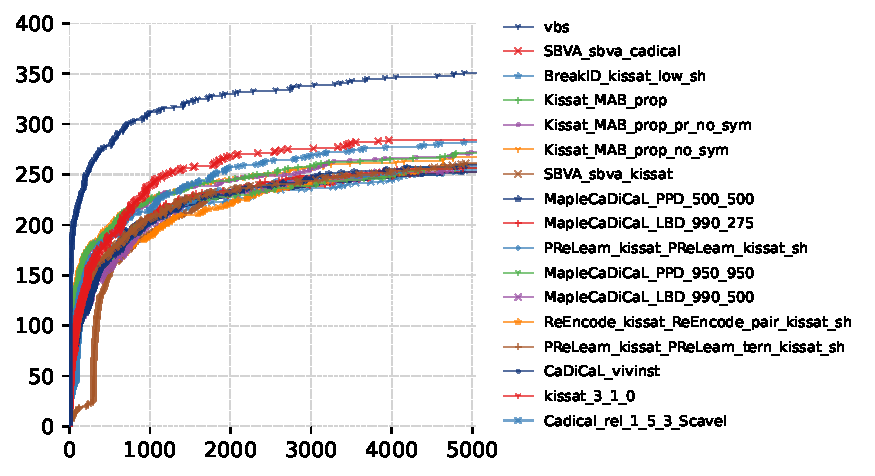
\includegraphics{gen/sc2023/cdf.pdf}
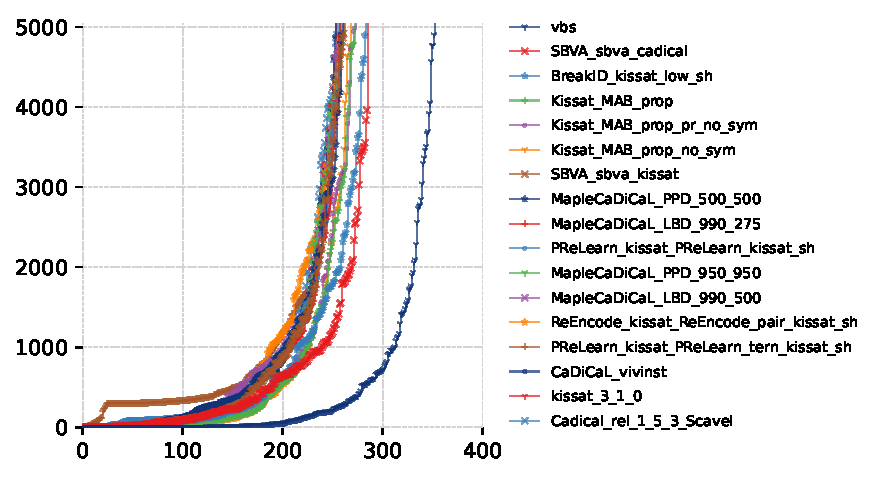
\includegraphics{gen/sc2023/cactus.pdf}


\section{SBVA-CaDiCaL vs. SBVA-Kissat}
\setlength{\tabcolsep}{.4em}
\begin{tabular}{lr|cc|c}
\toprule
Family & Count & SBVA CaDiCaL & SBVA Kissat & VBS \\
\midrule
Miscellaneous & 70 & 3071.07 & \bfseries 2779.72 & 2356.70 \\
Argumentation & 20 & 3693.93 & \bfseries 3477.05 & 3475.19 \\
Profitable-Robust-Production & 20 & \bfseries 2470.42 & 5058.18 & 2469.91 \\
Social-Golfer & 20 & \bfseries 7555.16 & 7690.23 & 7533.95 \\
Cryptography-Ascon & 20 & \bfseries 356.82 & 2811.89 & 324.37 \\
Set-Covering & 20 & 722.01 & \bfseries 345.13 & 238.27 \\
Hashtable-Safety & 20 & \bfseries 797.46 & 1396.84 & 797.46 \\
Interval-Matching & 20 & \bfseries 10000.00 & \bfseries 10000.00 & 10000.00 \\
Register-Allocation & 20 & 101.20 & \bfseries 95.28 & 61.05 \\
School-Timetabling & 19 & \bfseries 1399.65 & 2178.28 & 1187.72 \\
Brent-Equations & 19 & \bfseries 232.86 & 404.04 & 153.79 \\
Cryptography-Simon & 17 & \bfseries 10000.00 & \bfseries 10000.00 & 10000.00 \\
Grs-Fp-Comm & 17 & \bfseries 3649.90 & 4088.89 & 3647.53 \\
Satcoin & 15 & \bfseries 1395.53 & 10000.00 & 1395.53 \\
Mutilated-Chessboard & 12 & \bfseries 3194.54 & 4228.03 & 3194.54 \\
Tseitin & 11 & \bfseries 8196.91 & 8213.62 & 8196.74 \\
Miter & 11 & \bfseries 3134.91 & 4032.27 & 3105.64 \\
Pigeon-Hole & 8 & 5261.85 & \bfseries 5168.71 & 5168.70 \\
Hardware-Verification & 8 & 2832.05 & \bfseries 2714.99 & 2705.49 \\
Cryptography & 7 & 1578.46 & \bfseries 330.68 & 316.73 \\
Planning & 6 & \bfseries 6.97 & 7.75 & 6.49 \\
Quasigroup-Completion & 5 & 9.33 & \bfseries 6.49 & 6.12 \\
Reg-N & 5 & \bfseries 10000.00 & \bfseries 10000.00 & 10000.00 \\
Subsumptiontest & 5 & \bfseries 230.22 & 278.97 & 230.22 \\
Or\_Randxor & 5 & \bfseries 21.82 & 22.94 & 17.87 \\
\hline All & 400 & \bfseries 3257.62 & 3882.65 & 3051.46 \\
\bottomrule
\end{tabular}

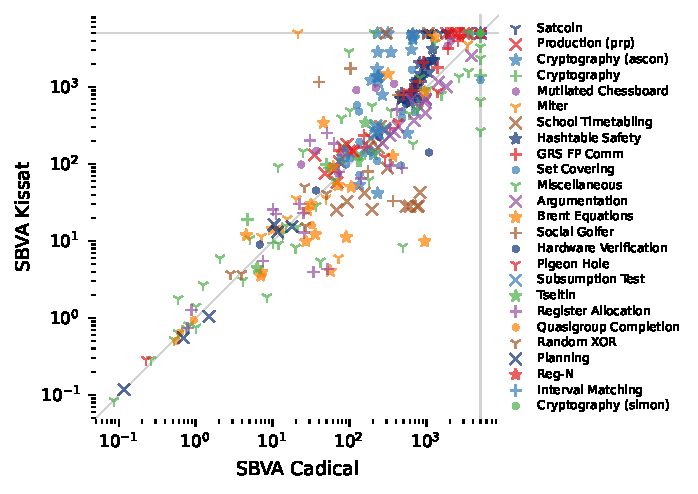
\includegraphics{gen/sc2023/sbva_cadical_kissat_logscale.pdf}

% \section{CaDiCaL-vivinst vs. Kissat-3.1.0}
% \begin{tabular}{lr|cc|c}
\toprule
Family & Count & Cadical\_Vivinst & Kissat\_3\_1\_0 & VBS \\
\midrule
Satcoin & 15 & 7388.71 & \bfseries 2495.86 & 2129.11 \\
Profitable-Robust-Production & 20 & \bfseries 2463.60 & 5024.62 & 2458.96 \\
Mutilated-Chessboard & 12 & \bfseries 2933.52 & 4131.55 & 2932.48 \\
Register-Allocation & 20 & \bfseries 8998.24 & 10000.00 & 8998.24 \\
Miter & 11 & \bfseries 3149.19 & 3710.41 & 3109.62 \\
School-Timetabling & 19 & \bfseries 1264.86 & 1669.03 & 1141.51 \\
Miscellaneous & 70 & 3140.29 & \bfseries 2779.33 & 2601.18 \\
Hashtable-Safety & 20 & \bfseries 460.96 & 805.04 & 458.63 \\
Social-Golfer & 20 & 7871.79 & \bfseries 7565.89 & 7564.08 \\
Grs-Fp-Comm & 17 & \bfseries 3659.80 & 3864.28 & 3632.29 \\
Argumentation & 20 & 3688.69 & \bfseries 3597.93 & 3566.72 \\
Set-Covering & 20 & 259.73 & \bfseries 174.42 & 149.20 \\
Pigeon-Hole & 8 & 6502.28 & \bfseries 6425.97 & 6412.68 \\
Cryptography-Ascon & 20 & 378.92 & \bfseries 303.29 & 284.36 \\
Brent-Equations & 19 & \bfseries 176.54 & 249.81 & 137.45 \\
Hardware-Verification & 8 & 2893.13 & \bfseries 2831.85 & 2755.54 \\
Cryptography & 7 & \bfseries 1602.26 & 1638.69 & 1582.76 \\
Subsumptiontest & 5 & \bfseries 46.47 & 76.98 & 25.46 \\
Tseitin & 11 & \bfseries 8201.03 & 8214.31 & 8199.91 \\
Planning & 6 & 13.03 & \bfseries 8.63 & 6.66 \\
Quasigroup-Completion & 5 & 2.70 & \bfseries 1.91 & 1.91 \\
Reg-N & 5 & \bfseries 10000.00 & \bfseries 10000.00 & 10000.00 \\
Interval-Matching & 20 & \bfseries 10000.00 & \bfseries 10000.00 & 10000.00 \\
Cryptography-Simon & 17 & \bfseries 10000.00 & \bfseries 10000.00 & 10000.00 \\
Or\_Randxor & 5 & \bfseries 10000.00 & \bfseries 10000.00 & 10000.00 \\
\hline All & 400 & \bfseries 4048.63 & 4050.74 & 3709.67 \\
\bottomrule
\end{tabular}

% 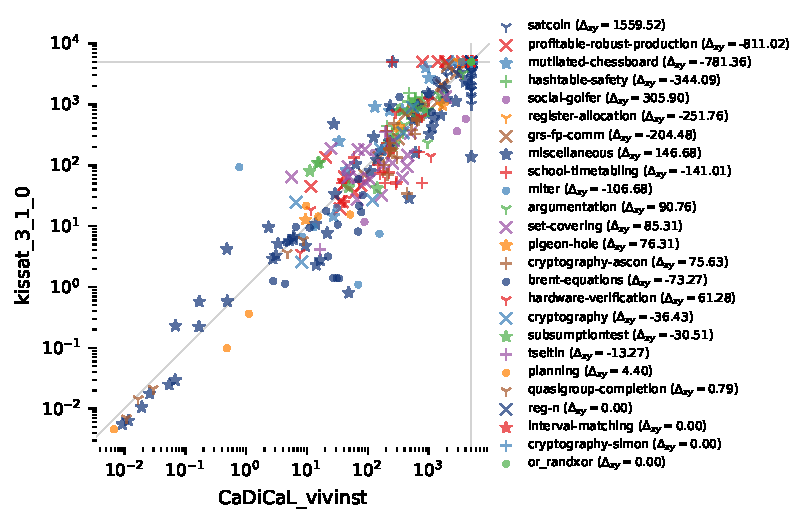
\includegraphics{gen/sc2023/Cadical_vivinst_Kissat_310_logscale.pdf}

% \section{SBVA-CaDiCaL vs. BreakId}
% \begin{tabular}{lr|cc|c}
\toprule
Family & Count & SBVA CaDiCaL & Breakid\_Kissat\_Low\_Sh & VBS \\
\midrule
Miscellaneous & 70 & 3071.07 & \bfseries 1964.08 & 1245.85 \\
Argumentation & 20 & 3693.93 & \bfseries 3447.39 & 3446.95 \\
Profitable-Robust-Production & 20 & \bfseries 2470.42 & 5031.37 & 2460.03 \\
Social-Golfer & 20 & \bfseries 7555.16 & 9013.05 & 7548.93 \\
Cryptography-Ascon & 20 & \bfseries 356.82 & 800.41 & 297.61 \\
Set-Covering & 20 & 722.01 & \bfseries 262.39 & 188.29 \\
Hashtable-Safety & 20 & \bfseries 797.46 & 1700.77 & 789.68 \\
Interval-Matching & 20 & \bfseries 10000.00 & \bfseries 10000.00 & 10000.00 \\
Register-Allocation & 20 & \bfseries 101.20 & 892.52 & 42.72 \\
School-Timetabling & 19 & \bfseries 1399.65 & 2371.42 & 1234.90 \\
Brent-Equations & 19 & \bfseries 232.86 & 698.16 & 168.16 \\
Cryptography-Simon & 17 & \bfseries 10000.00 & \bfseries 10000.00 & 10000.00 \\
Grs-Fp-Comm & 17 & \bfseries 3649.90 & 3865.34 & 3638.10 \\
Satcoin & 15 & \bfseries 1395.53 & 1421.87 & 1370.56 \\
Mutilated-Chessboard & 12 & \bfseries 3194.54 & 4240.09 & 3194.54 \\
Tseitin & 11 & 8196.91 & \bfseries 5772.63 & 5764.96 \\
Miter & 11 & \bfseries 3134.91 & 3143.29 & 3118.73 \\
Pigeon-Hole & 8 & 5261.85 & \bfseries 5128.03 & 5128.03 \\
Hardware-Verification & 8 & \bfseries 2832.05 & 2865.77 & 2717.96 \\
Cryptography & 7 & 1578.46 & \bfseries 1570.64 & 1554.56 \\
Planning & 6 & \bfseries 6.97 & 10.98 & 6.96 \\
Quasigroup-Completion & 5 & 9.33 & \bfseries 3.43 & 3.43 \\
Reg-N & 5 & \bfseries 10000.00 & \bfseries 10000.00 & 10000.00 \\
Subsumptiontest & 5 & 230.22 & \bfseries 89.14 & 89.14 \\
Or\_Randxor & 5 & \bfseries 21.82 & 103.93 & 21.82 \\
\hline All & 400 & \bfseries 3257.62 & 3376.88 & 2805.19 \\
\bottomrule
\end{tabular}

% 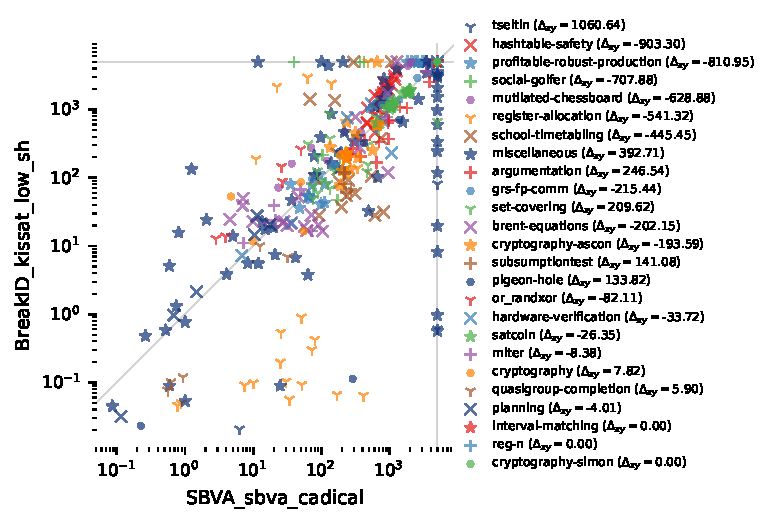
\includegraphics{gen/sc2023/sbva_cadical_breakid_logscale.pdf}

\section{Portfolio Analysis}

\begin{tabular}{l|p{.9\linewidth}r}
\toprule
K & Portfolio & Score \\
\midrule
1 & SBVA-CaDiCaL & 3257.62 \\
1 & BreakID-Kissat & 3376.88 \\
1 & KissatMABprop & 3575.78 \\
2 & BreakID-Kissat, KissatMABprop-pr-nosym & 2192.67 \\
2 & BreakID-Kissat, KissatMABprop-nosym & 2233.91 \\
2 & BreakID-Kissat, KissatMABprop & 2283.26 \\
3 & BreakID-Kissat, KissatMABprop-pr-nosym, CaDiCaL-Scavel & 2015.44 \\
3 & BreakID-Kissat, KissatMABprop-pr-nosym, SBVA-CaDiCaL & 2029.28 \\
3 & BreakID-Kissat, KissatMABprop-pr-nosym, MiniSat-XorEngine & 2030.71 \\
4 & BreakID-Kissat, KissatMABprop-pr-nosym, MiniSat-XorEngine, CaDiCaL-Scavel & 1853.78 \\
4 & BreakID-Kissat, KissatMABprop-pr-nosym, MiniSat-XorEngine, SBVA-CaDiCaL & 1867.67 \\
4 & BreakID-Kissat, KissatMABprop-pr-nosym, MiniSat-XorEngine, CaDiCaL-vivinst & 1876.50 \\
5 & BreakID-Kissat, KissatMABprop-pr-nosym, MiniSat-XorEngine, hKissatInc-unsat, CaDiCaL-Scavel & 1760.73 \\
5 & BreakID-Kissat, MiniSat-XorEngine, hKissatInc-unsat, CaDiCaL-Scavel, KissatMABprop-nosym & 1775.08 \\
5 & BreakID-Kissat, KissatMABprop-pr-nosym, MiniSat-XorEngine, hKissatInc-unsat, SBVA-CaDiCaL & 1777.68 \\
6 & BreakID-Kissat, KissatMABprop-pr-nosym, MiniSat-XorEngine, hKissatInc-unsat, CaDiCaL-Scavel, ReEncode-Kissat-pair & 1699.73 \\
6 & BreakID-Kissat, KissatMABprop-pr-nosym, MiniSat-XorEngine, hKissatInc-unsat, CaDiCaL-Scavel, AMSAT & 1701.04 \\
6 & BreakID-Kissat, KissatMABprop-pr-nosym, MiniSat-XorEngine, hKissatInc-unsat, CaDiCaL-Scavel, KissatMAB-Rephases & 1702.03 \\
7 & BreakID-Kissat, KissatMABprop-pr-nosym, MiniSat-XorEngine, hKissatInc-unsat, CaDiCaL-Scavel, AMSAT, KissatMAB-Rephases & 1662.14 \\
7 & BreakID-Kissat, KissatMABprop-pr-nosym, MiniSat-XorEngine, hKissatInc-unsat, CaDiCaL-Scavel, AMSAT, ReEncode-Kissat-pair & 1663.30 \\
7 & BreakID-Kissat, KissatMABprop-pr-nosym, MiniSat-XorEngine, hKissatInc-unsat, CaDiCaL-Scavel, CaDiCaL-vivinst, KissatMAB-Rephases & 1663.99 \\
\bottomrule
\end{tabular}

\setlength{\tabcolsep}{.4em}
\begin{tabular}{lr|>{\raggedleft\arraybackslash}p{0.15\linewidth}>{\raggedleft\arraybackslash}p{0.15\linewidth}>{\raggedleft\arraybackslash}p{0.15\linewidth}|>{\raggedleft\arraybackslash}p{0.15\linewidth}}
\toprule
Family & \# & BreakId Kissat & KissatMAB PropPrNos & Cadical Scavel & VBS \\
\midrule
Interval Matching & 20 & $10000.00$ & \bfseries $0.15$ & $10000.00$ & $0.15$ \\
Random XOR & 5 & \bfseries $103.93$ & $10000.00$ & $10000.00$ & $17.87$ \\
Register Allocation & 20 & $892.52$ & \bfseries $5.50$ & $9135.93$ & $1.61$ \\
Satcoin & 15 & \bfseries $1421.87$ & $10000.00$ & $7446.36$ & $1151.09$ \\
Set Covering & 20 & $262.39$ & $5761.57$ & \bfseries $218.58$ & $2.88$ \\
Cryptography (ascon) & 20 & $800.41$ & $5628.35$ & \bfseries $404.02$ & $234.84$ \\
Reg-N & 5 & $10000.00$ & \bfseries $6295.16$ & $10000.00$ & $4766.27$ \\
Mutilated Chessboard & 12 & $4240.09$ & \bfseries $1656.50$ & $3138.80$ & $1540.17$ \\
Production (prp) & 20 & $5031.37$ & $3946.63$ & \bfseries $2468.35$ & $1333.87$ \\
Tseitin & 11 & \bfseries $5772.63$ & $8193.40$ & $8199.26$ & $249.27$ \\
Hashtable Safety & 20 & $1700.77$ & \bfseries $194.75$ & $478.24$ & $179.58$ \\
Social Golfer & 20 & $9013.05$ & $7665.62$ & \bfseries $7522.35$ & $5654.50$ \\
Pigeon Hole & 8 & \bfseries $5128.03$ & $6381.16$ & $6482.43$ & $5063.78$ \\
Hardware Verification & 8 & $2865.77$ & \bfseries $1558.52$ & $2851.32$ & $1443.63$ \\
School Timetabling & 19 & $2371.42$ & \bfseries $1266.09$ & $2345.57$ & $1087.90$ \\
Miscellaneous & 70 & \bfseries $1964.08$ & $2470.82$ & $2921.43$ & $490.37$ \\
Argumentation & 20 & \bfseries $3447.39$ & $4144.27$ & $3698.40$ & $3401.26$ \\
Brent Equations & 19 & $698.16$ & $408.33$ & \bfseries $154.07$ & $83.28$ \\
GRS FP Comm & 17 & $3865.34$ & \bfseries $3435.82$ & $3752.92$ & $1885.76$ \\
Cryptography (simon) & 17 & $10000.00$ & $10000.00$ & \bfseries $9700.12$ & $9700.12$ \\
Cryptography & 7 & \bfseries $1570.64$ & $1577.96$ & $1661.79$ & $269.45$ \\
\hline All & 400 & \bfseries $3376.88$ & $3580.43$ & $4050.95$ & $1548.15$ \\
\bottomrule
\end{tabular}


% \section{Family-wise CDF Plots}
% 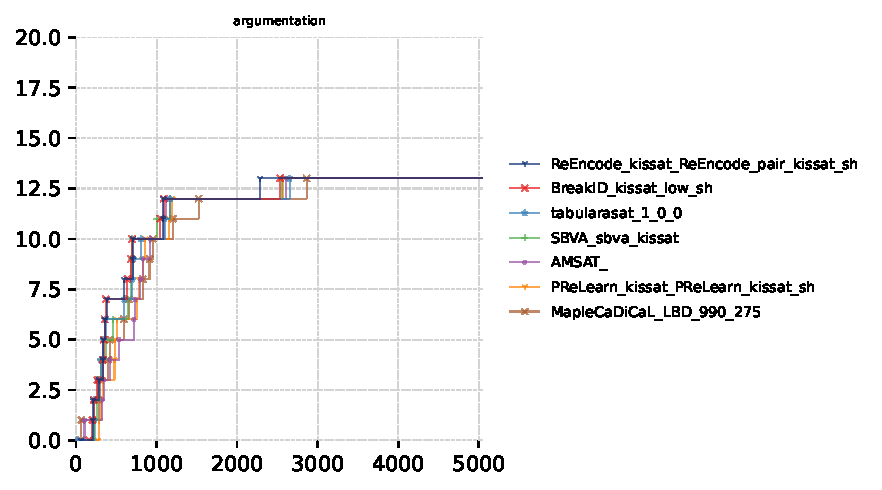
\includegraphics[width=\linewidth]{gen/sc2023/cdfs/cdf-argumentation.pdf}
% 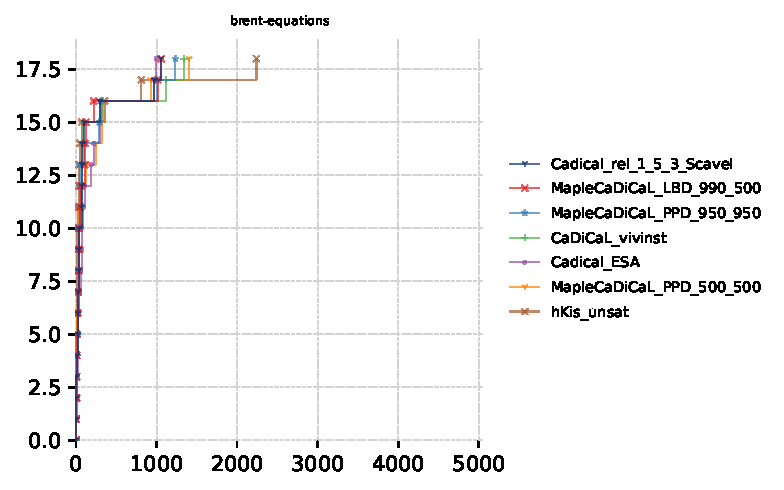
\includegraphics[width=\linewidth]{gen/sc2023/cdfs/cdf-brent-equations.pdf}
% 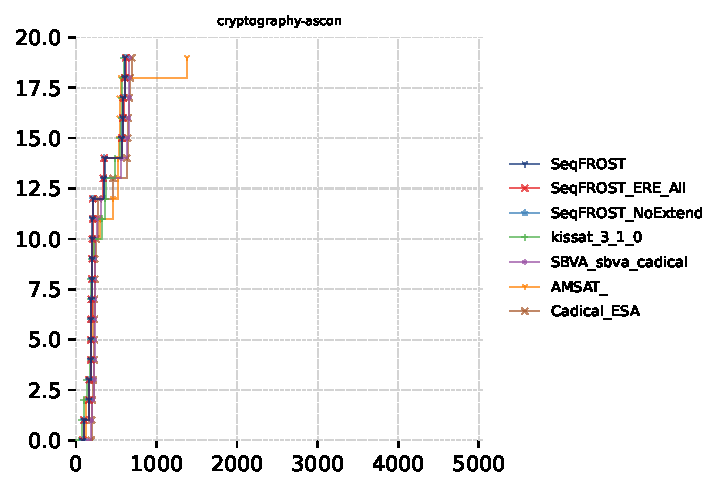
\includegraphics[width=\linewidth]{gen/sc2023/cdfs/cdf-cryptography-ascon.pdf}
% 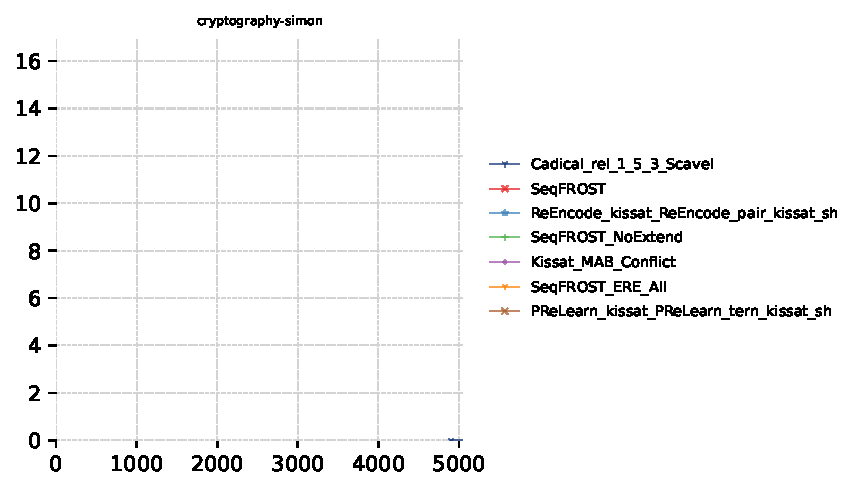
\includegraphics[width=\linewidth]{gen/sc2023/cdfs/cdf-cryptography-simon.pdf}
% 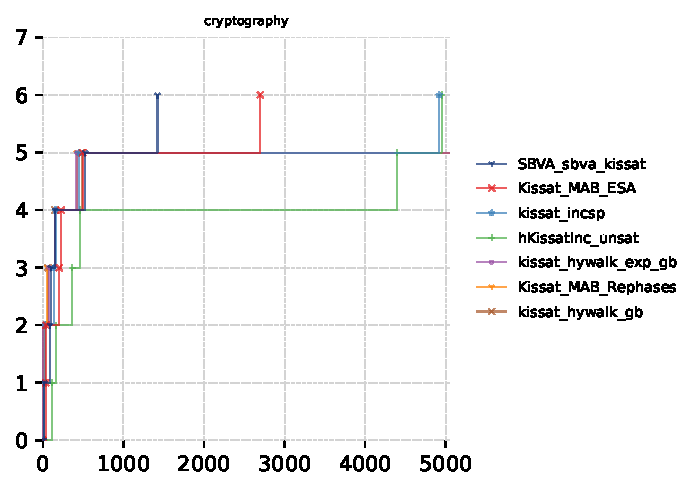
\includegraphics[width=\linewidth]{gen/sc2023/cdfs/cdf-cryptography.pdf}
% 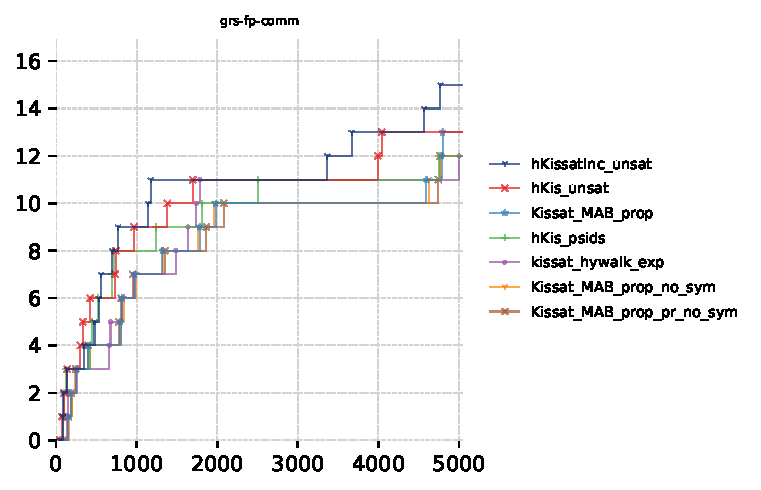
\includegraphics[width=\linewidth]{gen/sc2023/cdfs/cdf-grs-fp-comm.pdf}
% 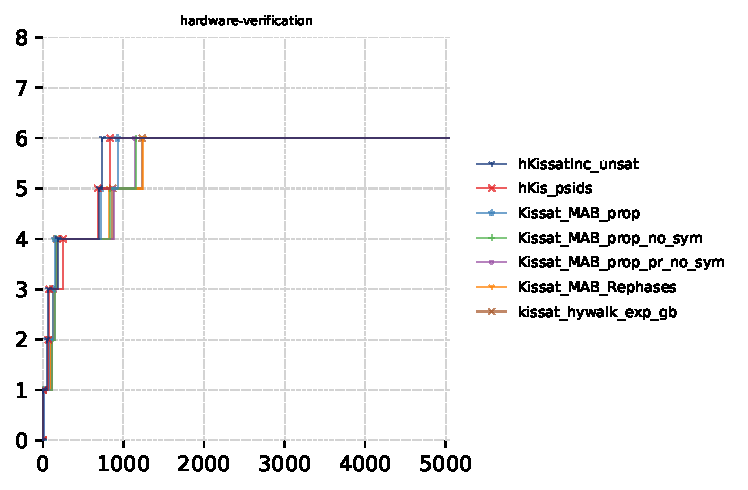
\includegraphics[width=\linewidth]{gen/sc2023/cdfs/cdf-hardware-verification.pdf}
% 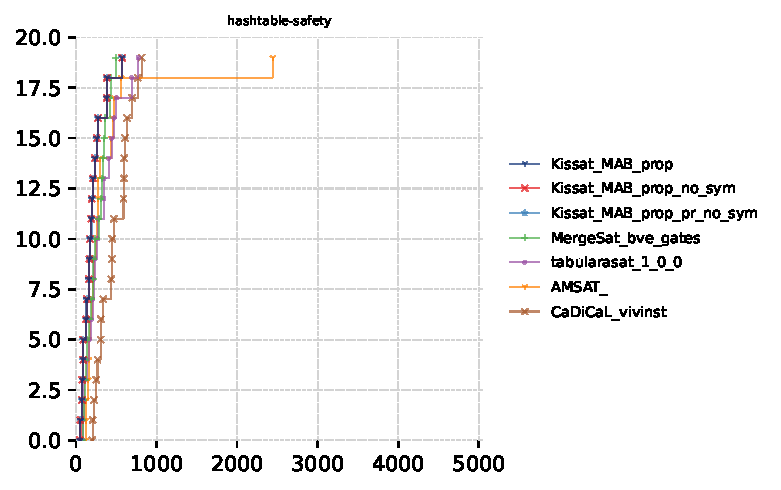
\includegraphics[width=\linewidth]{gen/sc2023/cdfs/cdf-hashtable-safety.pdf}
% 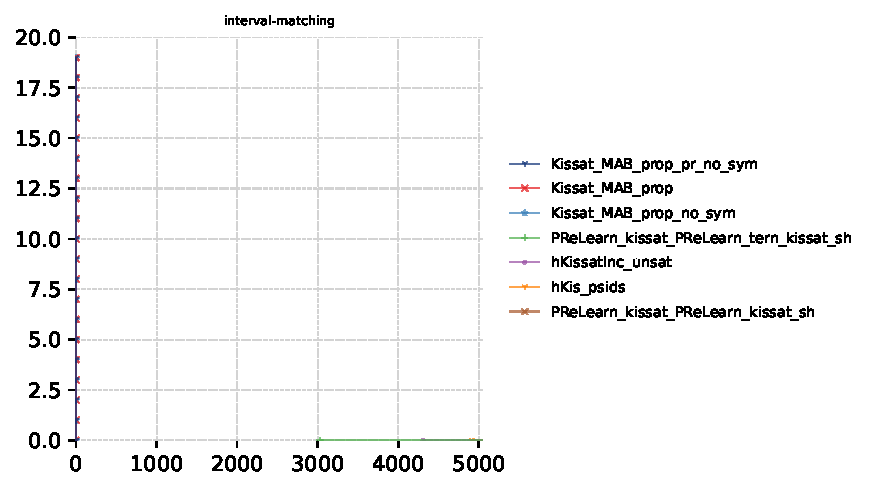
\includegraphics[width=\linewidth]{gen/sc2023/cdfs/cdf-interval-matching.pdf}
% 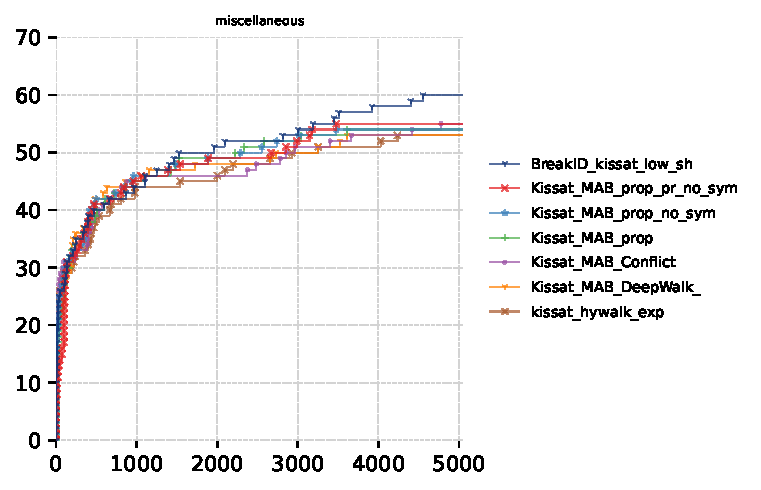
\includegraphics[width=\linewidth]{gen/sc2023/cdfs/cdf-miscellaneous.pdf}
% 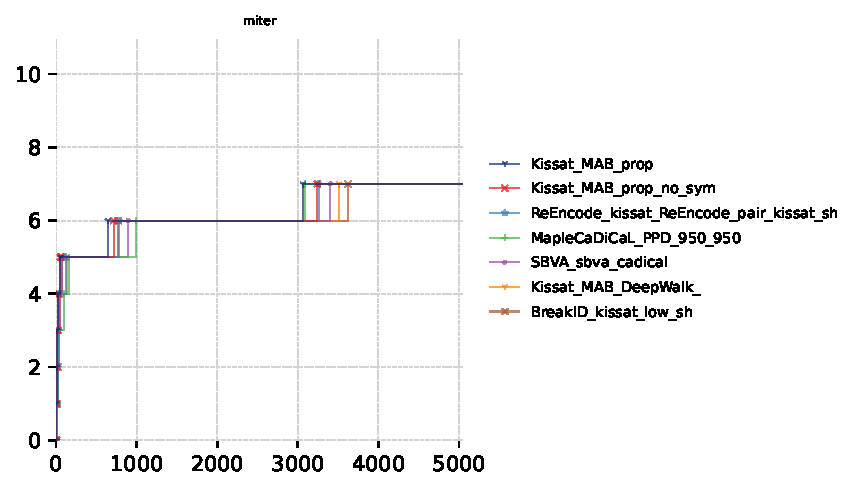
\includegraphics[width=\linewidth]{gen/sc2023/cdfs/cdf-miter.pdf}
% 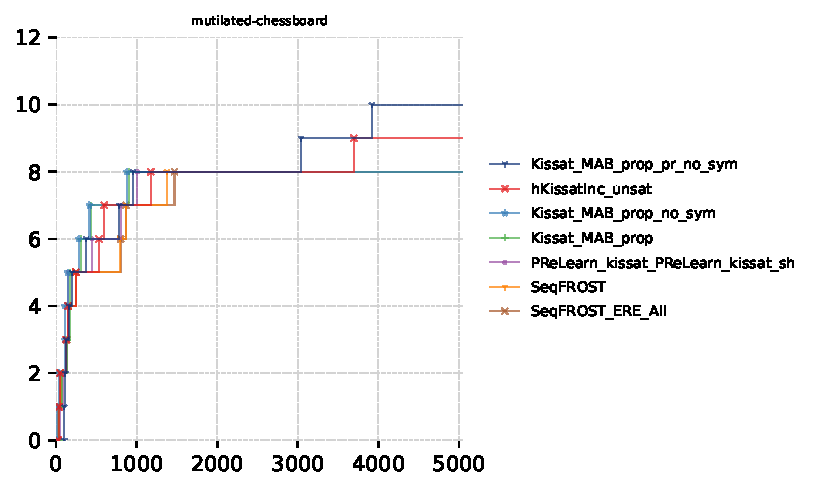
\includegraphics[width=\linewidth]{gen/sc2023/cdfs/cdf-mutilated-chessboard.pdf}
% 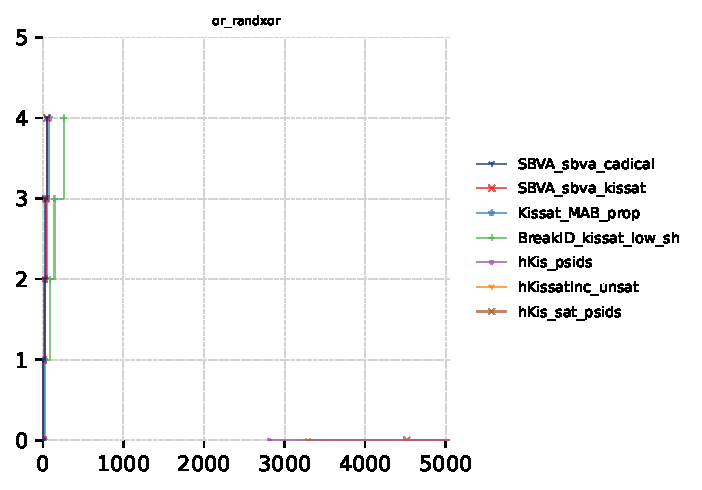
\includegraphics[width=\linewidth]{gen/sc2023/cdfs/cdf-or_randxor.pdf}
% 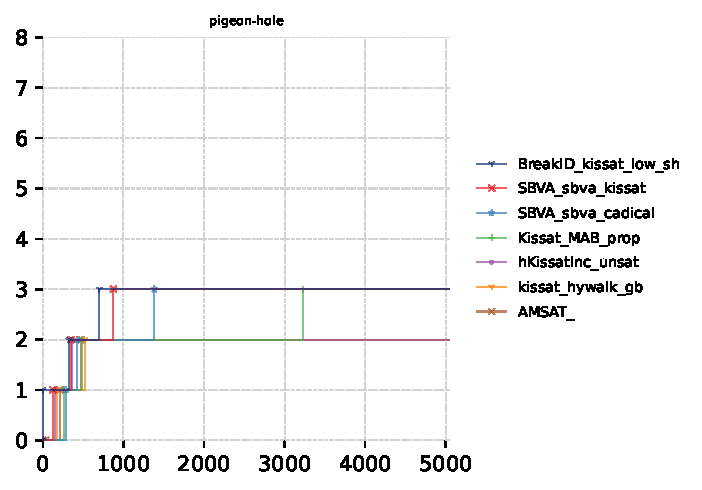
\includegraphics[width=\linewidth]{gen/sc2023/cdfs/cdf-pigeon-hole.pdf}
% 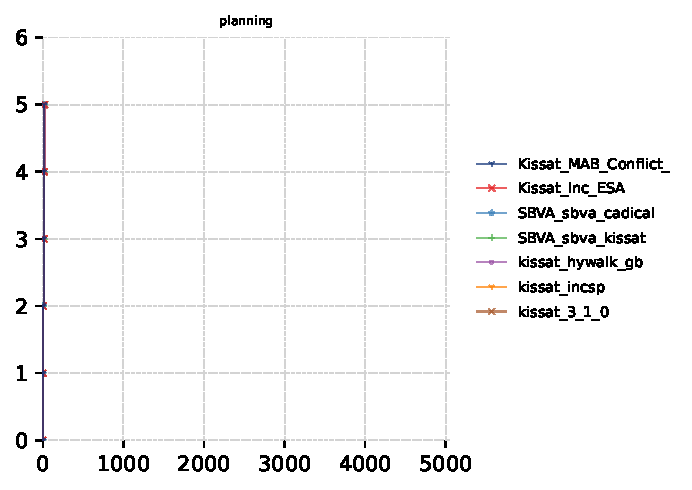
\includegraphics[width=\linewidth]{gen/sc2023/cdfs/cdf-planning.pdf}
% 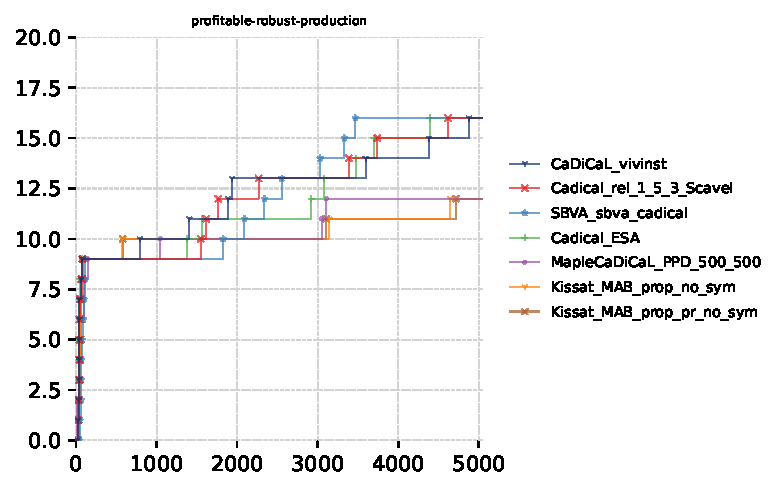
\includegraphics[width=\linewidth]{gen/sc2023/cdfs/cdf-profitable-robust-production.pdf}
% 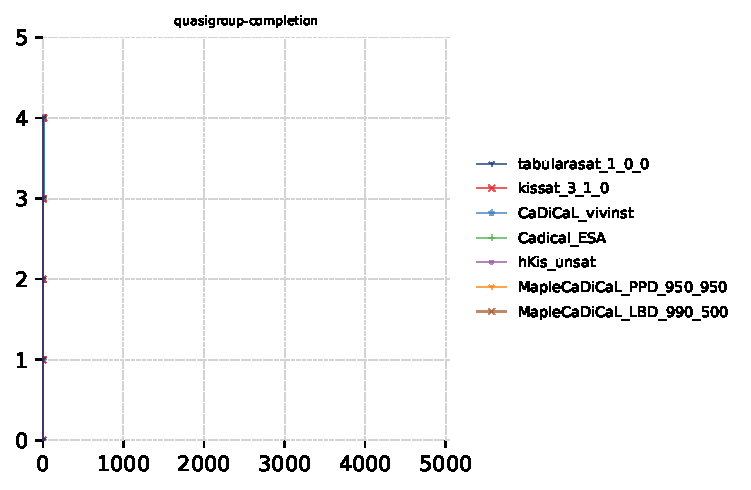
\includegraphics[width=\linewidth]{gen/sc2023/cdfs/cdf-quasigroup-completion.pdf}
% 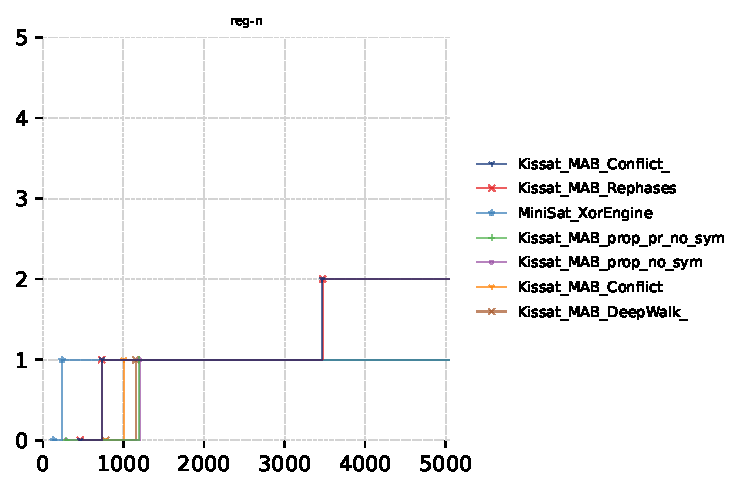
\includegraphics[width=\linewidth]{gen/sc2023/cdfs/cdf-reg-n.pdf}
% 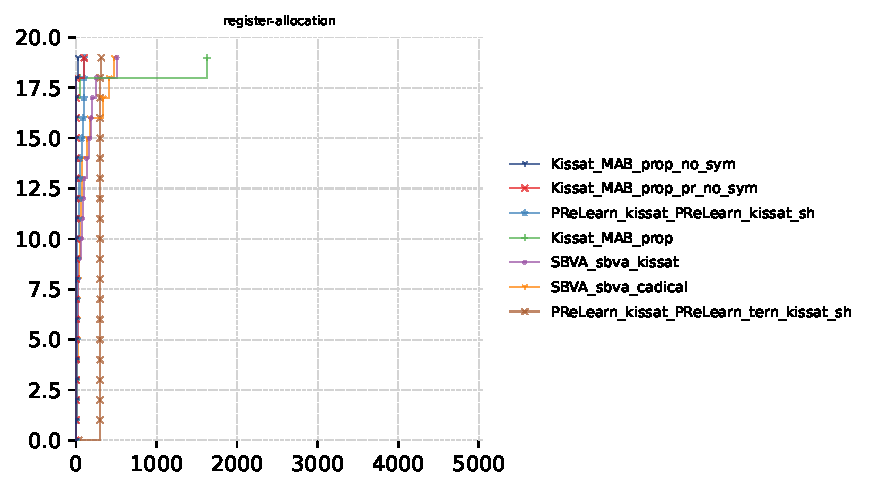
\includegraphics[width=\linewidth]{gen/sc2023/cdfs/cdf-register-allocation.pdf}
% 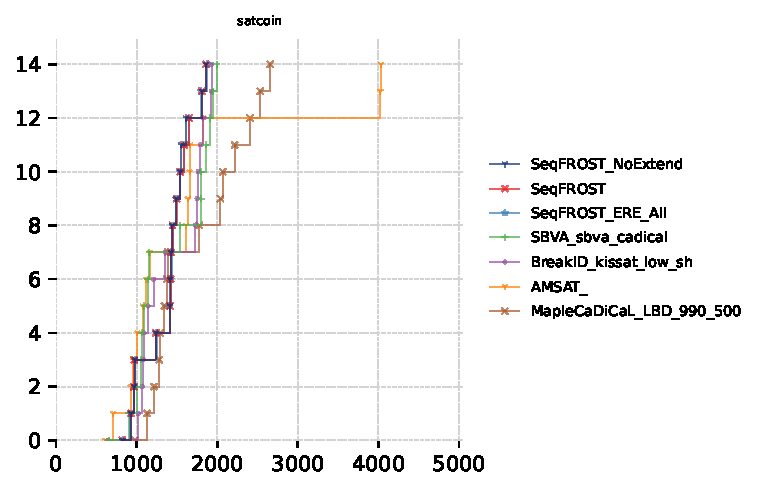
\includegraphics[width=\linewidth]{gen/sc2023/cdfs/cdf-satcoin.pdf}
% 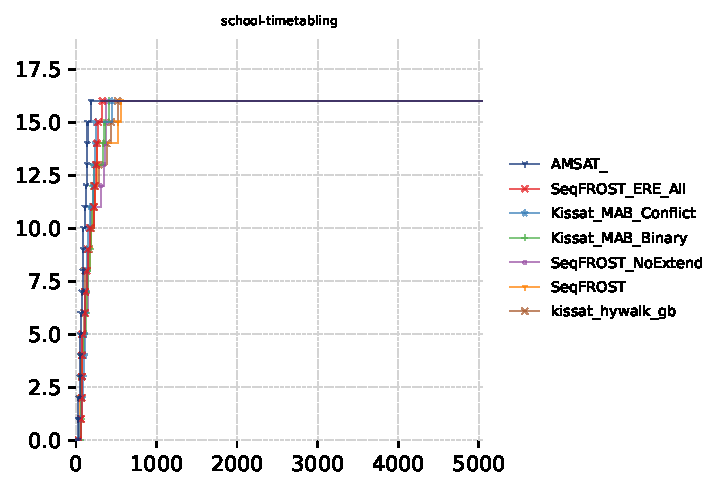
\includegraphics[width=\linewidth]{gen/sc2023/cdfs/cdf-school-timetabling.pdf}
% 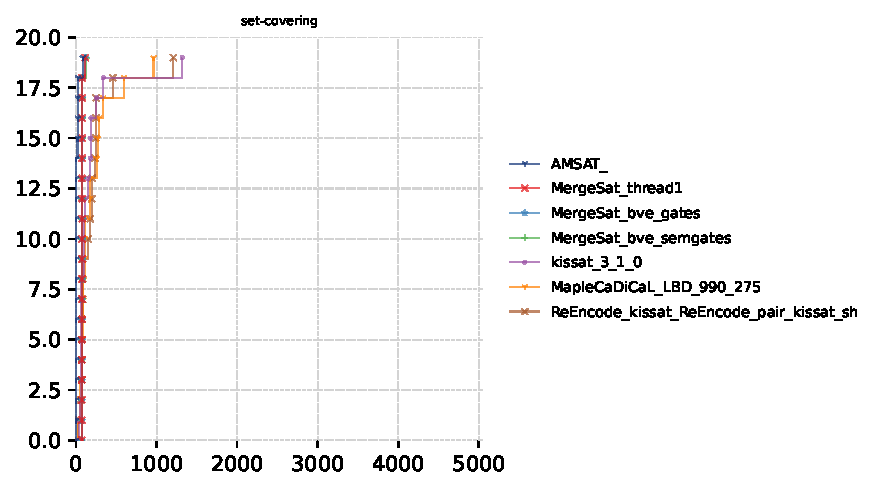
\includegraphics[width=\linewidth]{gen/sc2023/cdfs/cdf-set-covering.pdf}
% 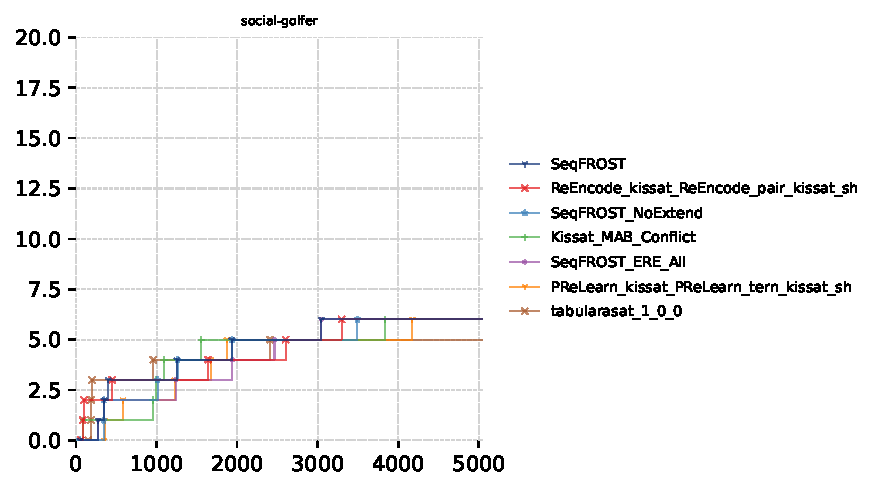
\includegraphics[width=\linewidth]{gen/sc2023/cdfs/cdf-social-golfer.pdf}
% 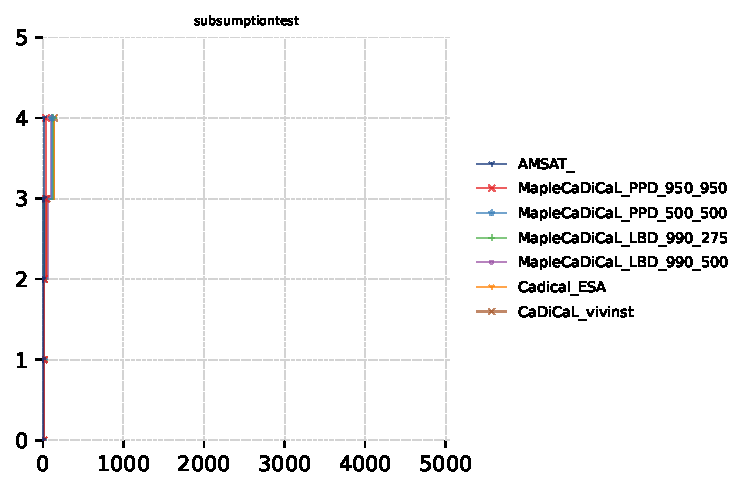
\includegraphics[width=\linewidth]{gen/sc2023/cdfs/cdf-subsumptiontest.pdf}
% 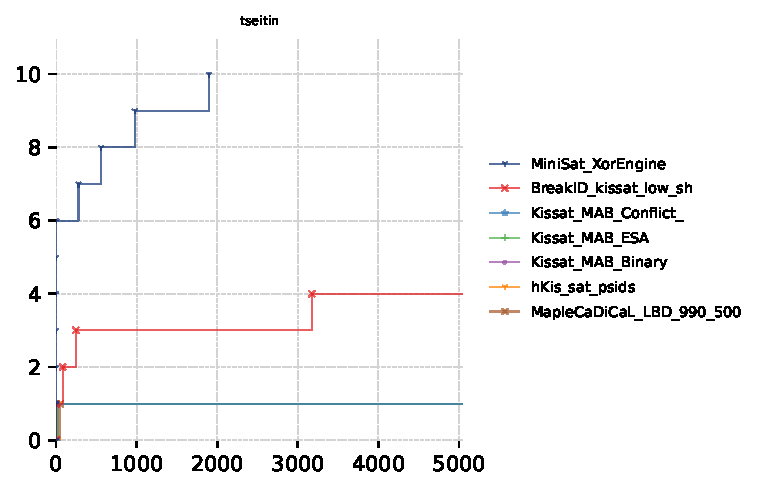
\includegraphics[width=\linewidth]{gen/sc2023/cdfs/cdf-tseitin.pdf}


\end{document}